\chapter{Generators}
\section{Iterators}
Before getting into generators, we need to define iterators first. Iterators, as their name suggests, represent a state of iteration of some sequence backed by either themselves or some other object. In both C\# and PHP, they can be arbitrary objects implementing an \emph{Iterator}\footnote{\citep{IterPHP}} (for PHP) or an \emph{IEnumerator}\footnote{\citep{IterNet}} (in C\#) interface. 

Both of these contain a number of methods  (\autoref{fig1.1:iterators}). However, for now we will focus only on two of them that they both share, \emph{current} and \emph{next}. The first one - \emph{current} - should always return the element the iterator is currently pointing at. As such, it should never modify the state of the iterator and should generally be free of side effects. The second one - \emph{next} - should advance the iterator to the next item, effectively changing what element the \emph{current} method returns.

\begin{figure}[h]	
	\centering	
	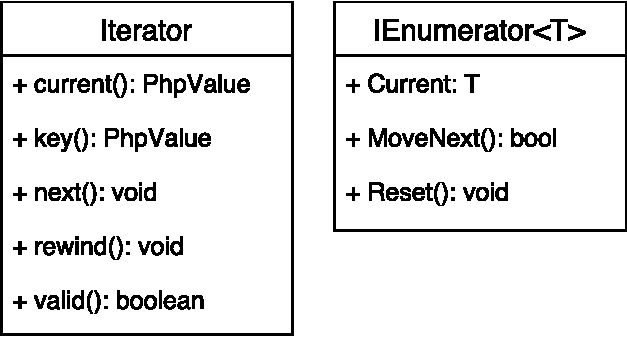
\includegraphics[scale=0.75]{../img/1_1_iterators}	
	\caption{Iterator and IEnumerable interfaces.}
	\label{fig1.1:iterators}
\end{figure}

Iterators serve, among other things, as a useful tool to handle large sequences of items. Instead of generating everything at once and then keeping it, for example, in an array, one can simply create an iterator that generates and serves the elements one by one. This enables a lower memory footprint, because there is never need to keep all the elements in memory at once. 

Furthermore, instead of spending a lot of resources at once in the beginning to create the whole sequence, the iterator can now spend considerably fewer for each element’s creation when the \emph{next} method is called. Though the final price is the same regardless it enables a more even distribution of the performance hit. Also, one does not need to pay for the elements that do not get created - the ones that are not iterated over.

There is one problem with iterators, however. They are fairly tedious to write. The main issue stems from the fact that unlike in a normal method in which you would create the whole sequence at once, in the iterator’s \emph{next} method you always need to explicitly save and then retrieve the current state of the execution. There is a lot of boilerplate associated with them as well. You need to create a new type and implement a number of methods that do not actually do anything useful.

To give an example (\autoref{list1.1:iterator}), creating an array of numbers $1$ to $n$ is a straightforward for loop with an assignment. In the case of an iterator’s \emph{next} method, you need to first retrieve the last used number, increase it by one, and then store it. You also need to implement a \emph{current} method that returns the last stored index and a few other ones that are essentially just a busywork. 

\begin{listing}[H]
	\caption{Method that creates everything at once and as an Iterator.}
	\label{list1.1:iterator}
\begin{minted}{php}
<?php
function by_one_at_once(){
  $result = [];
  for($i = 0; $i < 10; $i++){
    $result[] = $i;
  }
  return $result;
}

class byOneIterator implements Iterator {
  private $position = 0;

  public function rewind() {$this->position = 0;}
  public function key() {return $this->position;}
  public function current() {return $this->position; }
  public function next() {
  $curr_pos = $this->position;
    $curr_pos += 1;
    $this->position = $curr_pos;
  }
  public function valid(){ return ($this->position < 10); }
}
\end{minted}
\end{listing}

While for a monotone sequence of numbers even the iterator is still simple and readable, this quickly ceases to be the case with a higher complexity of the iteration. The amount of code needed for state keeping increases quite quickly and an algorithm, which would otherwise be really straightforward when used for the creation of the whole sequence at once, becomes convoluted. This is where generators emerge as a relevant solution.


\section{Generators universally}

Generators provide an easy way to write methods that return iterators while the code can be almost the same as if they returned whole sequences at once instead. All the transforming of the algorithm into the \emph{next} method with its retrieving of the last state in the beginning and state saving after a new element gets set as \emph{current} is handled transparently for the programmer. There is also no need to create a new type and implement other iterator’s busywork methods with them. They automatically return correct and fully implemented iterators.

To achieve this, a new keyword \emph{yield} or \emph{yield return} is usually introduced. It serves two purposes. First, it marks the spots where the \emph{next} method of the returned iterator should stop executing and save the current state. Second, much like the \emph{return} keyword, it specifies a value being returned - in this case actually a value that should be set as \emph{current} on the iterator.

To continue with our example of creating a sequence of numbers from $1$ to $n$ (\autoref{list1.1:generator}), one would write a generator method the same way as a normal method generating the whole array, the only difference being that instead of an assignment into a result array, the for loop would contain a \emph{yield} of the current index. 

\begin{listing}[H]
	\caption{By one sequence as a generator.}
	\label{list1.1:generator}
\begin{minted}{php}
<?php
function by_one_generator(){
  for($i = 0; $i < 10; $i++){
    yield $i;
  }
}
\end{minted}
\end{listing}

An iterator returned from such a generator method (\autoref{fig1.2:generator}) would have a \emph{next} method that would always start from the last encountered \emph{yield}, execute update and condition part of the for loop, and then set a new element as the \emph{current} one.

\begin{figure}[h]
	\centering	
	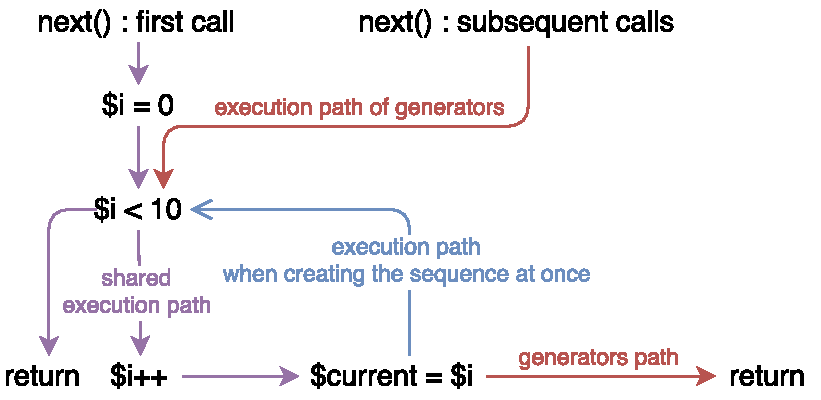
\includegraphics[scale=0.75]{../img/1_2_generators}	
	\caption{Generator's control flow graph.}
	\label{fig1.2:generator}
\end{figure}

\section{Generators in PHP}

Generators in PHP are not just about creating data, however. They support consuming data as well (\autoref{list1.1:yieldLogger}). Namely, one can send an arbitrary value into the returned iterator through its method called \emph{send}. This method takes one argument - the value being sent, sets it as a result of the last \emph{yield} expression, and resumes the evaluation the same way as the \emph{next} method would.

\begin{listing}[H]
	\caption{Generator method used as a logger.}
	\label{list1.1:yieldLogger}
\begin{minted}{php}
<?php
function logger_generator(){
  $logger = new Logger();
  while(($line = yield) != "END"){
    $logger->log($line);
  }
  $logger->close();
}
class Logger{
  public function close(){ echo "END;";}
  public function log($line){ echo $line; }
}

$gen = logger_generator();
$gen->send("First!");
$gen->send("Second!");
$gen->send("END");
\end{minted}
\end{listing}

This means that unlike in C\#, where \emph{yield} is a statement and therefore can not be a part of a bigger computation or a function call, in PHP \emph{yield} can be literally anywhere, even in the place of a function call argument. This further complicates the state saving. In addition to all the local variables, when \emph{yield} is part of some bigger expression, we need to save its state as well. Moreover, it needs to be done the right way to ensure a correct order of execution.

Due to various design reasons, \citep{CSharpYieldFinaly} C\# also limits where \emph{yields} can happen with regards to exception control blocks. They are not allowed in \emph{catch}\footnote{\citep{CSharpYieldCatch}} and \emph{finally} blocks\footnote{\citep{CSharpYieldFinaly}} altogether and can only be in \emph{try} blocks\footnote{\citep{CSharpYieldTry}} that do not have any associated catch blocks. PHP, on the other hand, allows yielding everywhere, be it in \emph{try}, \emph{catch}, or \emph{finally} blocks.

\section{Generators in other languages}

These limitations are not unique to C\#, however. Both F\# and Visual Basic, the only other truly mainstream CIL based languages, also support generators with these restrictions. For them, \emph{yield} is just a statement that can not appear in certain exception handling blocks.

In fact, \emph{yield} being an expression holding a send value is not even a feature all dynamic languages share. JavaScript, for example, merely briefly supported {\citep{ECMAYield}} such behavior and as of ECMA 2015 has \emph{yield} only as a statement.

That, nonetheless, does not mean that PHP is completely unique with regards to generators. In Python\footnote{\citep{PythonYield}}, another mainly interpreted dynamic language, \emph{yields} are expressions and are allowed in exception handling blocks almost the same way as in PHP. In Lua\footnote{\citep{LUAYield}} they are implemented as a special version of coroutines and thus have an even wider set of features.




